\documentclass[../main]{subfiles}

\graphicspath{{../figures/}}

\begin{document}

\section{屋内実験} \label{sec:indoor_experiment}

本研究では,屋内環境においてプラント内を模擬した実験セットアップを構築し,提案手法の有効性を検証した.
まず実験環境と装置構成について説明し,その後,実験結果と考察を示す.

\subsection{実験環境} \label{subsec:vexp_ref_environmet}

本実験で用いた環境は,図\ref{fig:exp_setup}に示すように,研究室内に作業台やARマーカーを配置し,複数の小型ギアボックスを設置し,
それぞれの機器の稼働音が重なり合う騒音のある状況を再現したものである.
このような手法によって,石油精製プラントなどの産業施設を想定した雑音下での異常音検知を屋内で模擬できるようにしている.
\begin{figure}[t]
  \centering
  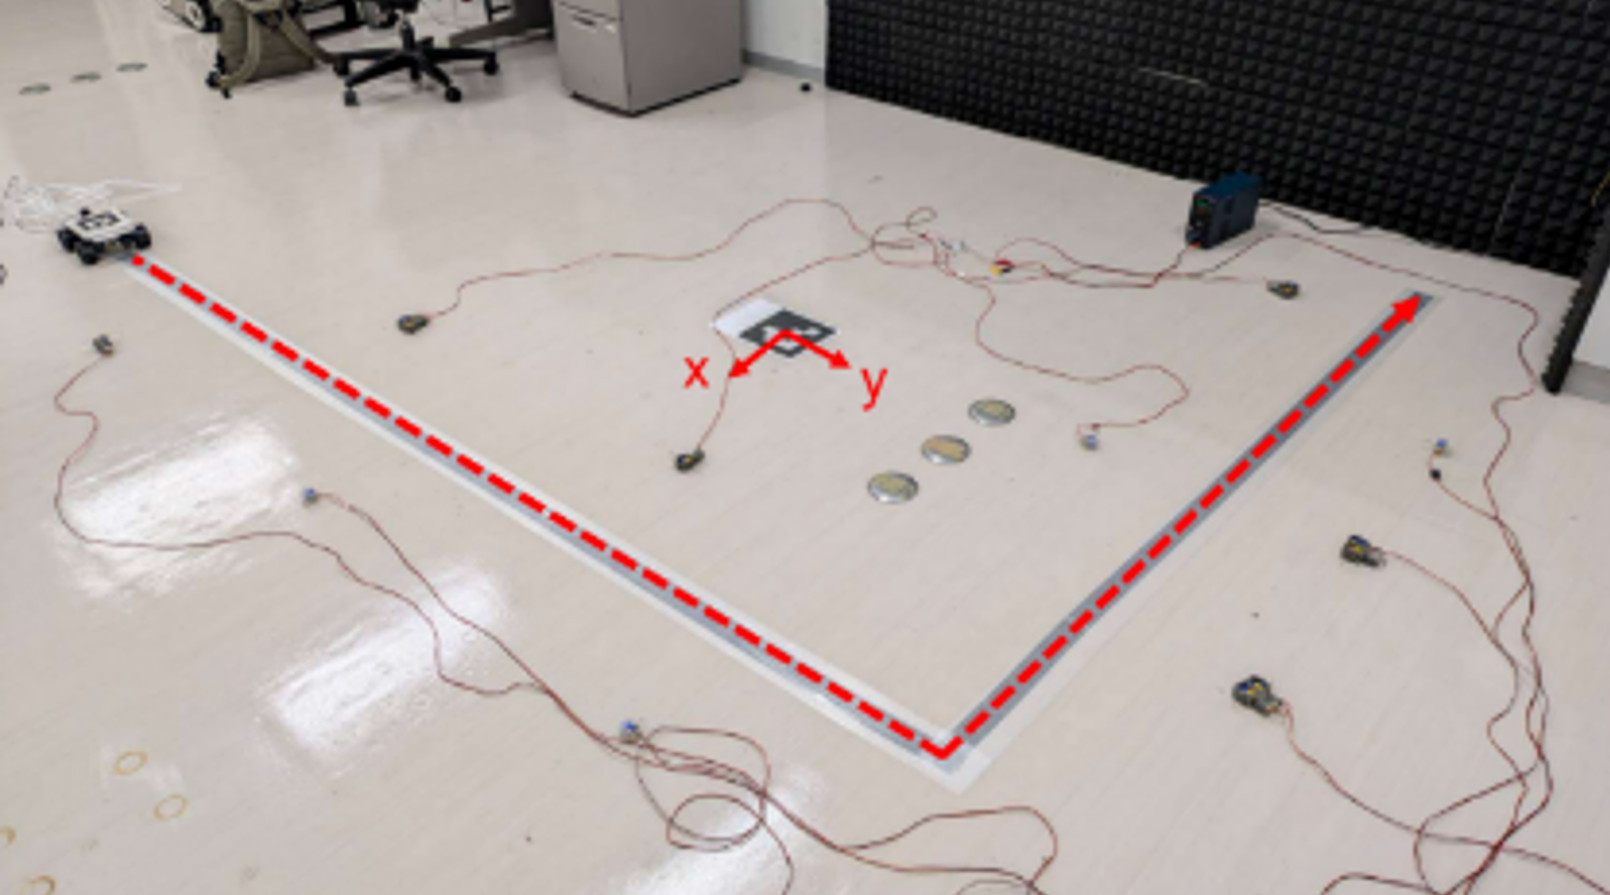
\includegraphics[keepaspectratio, width=0.7\linewidth]{chap4/env_experiment.png}
  \caption{実験環境}
  \label{fig:exp_setup}
\end{figure}


\subsubsection{機器構成} \label{subsubsec:device_config}

小型の移動ロボットを用い,その上にマイクロホンを搭載して実際の配管や機器周囲を巡回する点検作業を想定した.
音響信号はShure SM11マイクロホンとZoom P4を接続し,48kHzで取得する.
またARマーカーを用いてLogicool C925eカメラで位置情報を追跡し,
経路全体を俯瞰することで,ロボットの移動経路上で得られる音響情報と空間情報を同時に記録可能にした.

\subsubsection{移動ロボットの位置推定}
位置情報取得は,ARマーカーを2つ用いて行った.
1つは基準となる座標系として使用し,もう1つはロボットに搭載して使用する.
これらのARマーカーをArucoライブラリを用いて認識することで,
カメラ座標系からそれぞれのマーカーへの同次変換行列を取得することができる\cite{aruco2014}.
次に,カメラ座標系から見たロボット座標系の位置を推定するために,これらの同次変換行列を合成することで,ロボットの位置を推定した.
基準座標系を原点としたロボットの位置を推定することで,カメラの姿勢のずれに頑強な位置推定を実現した.
\subsubsection{騒音環境のシミュレーション} \label{subsubsec:noise_simulation}
騒音環境を再現するために,タミヤ製教育工作キットのギアボックスを複数種類用意し,簡易的な回転機器を模した状態にしている.
\reffig{fig:gearbox}に本実験にて使用した3種類のギアボックスを示す.


\begin{figure}[t]
  \centering
  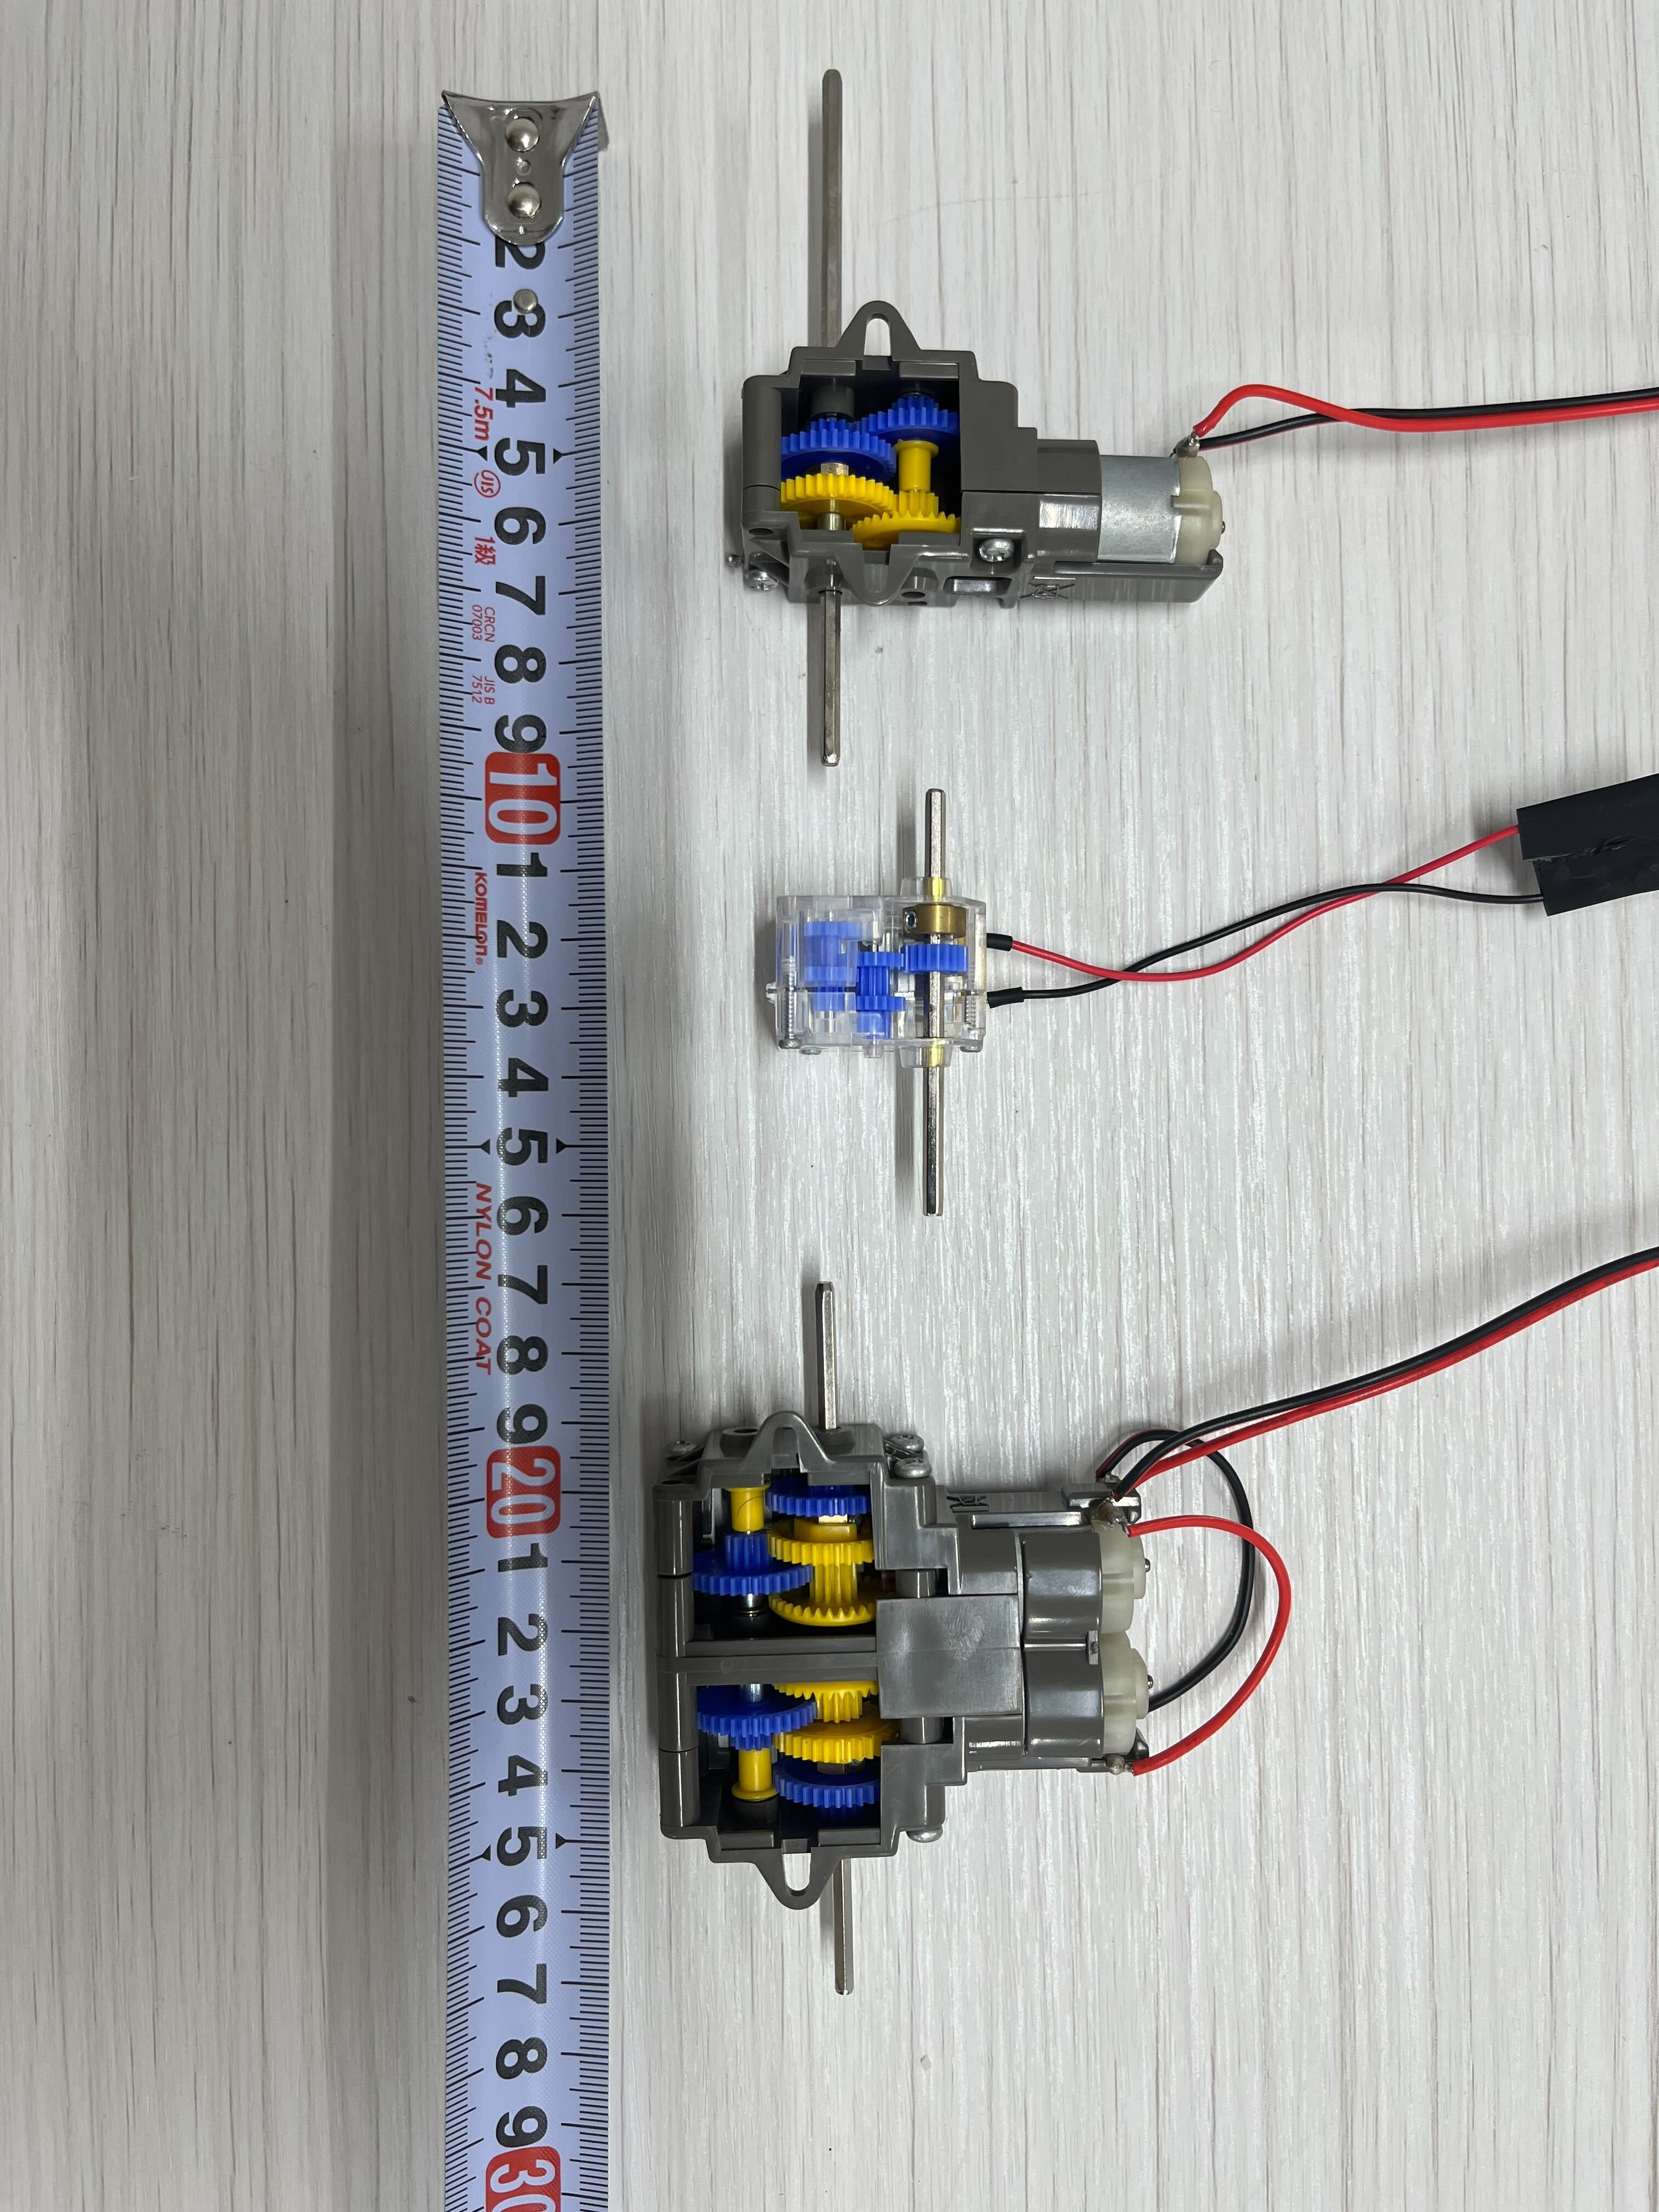
\includegraphics[angle=90,keepaspectratio, width=0.7\linewidth]{chap4/gearbox.jpg}
  \caption{音源のギアボックス}
  \label{fig:gearbox}
\end{figure}

ギアボックスを本実験の音源として用いた理由は,プラント内における音響点検において,音響点検の主な対象となる機器がポンプなどの回転機器であり,
これら回転機器から発せられる音は\refsec{sec:pmethod_mapping}で述べたように,一定の動作条件下では,周波数領域において定常的な特徴を持つことが知られている.
提案手法では,この全ての音源が定常的な特徴を持つという仮定の下,正常音の学習を行っているため,
同様に回転機器であり,稼働中に発する音に定常的な特徴を持つギアボックスを音源として用いている.

また,これらのギアボックスは傾けるとギア同士が強く擦れ合って研削音を生じるため,異常音を発生させることが可能である.
\subsubsection{データの前処理} \label{subsec:data_preprocessing}
マイクロホンを用いて録音したデータ内の低周波帯において,移動ロボットの振動によるものと思われるノイズが含まれていたため,
このノイズに対応すると思われる1000Hz未満に対応する周波数帯域を除去した.
また,メルスペクトログラムへの変換においては,突発的なノイズによる特徴量の不安定化を防ぐために,短時間フーリエ変換に用いるウィンドウ幅を一般に使用されるウィンドウ幅よりもかなり大きい65536サンプルに設定した.
48kHzで音響信号を取得しているため,これは約1.36秒のウィンドウ幅に相当する.
\subsection{実験手順} \label{subsec:experiment_procedure}

本実験では,まずすべてのギアボックスを正常に動作させた状態でロボットを走行させ,正常サンプルを収集した.
続いて,1つのギアボックスを傾けて異常音を発生させ,ロボットを同様に走行させることで異常サンプルを取得している
異常状態における走行は,異常音源の位置を変えて2回行い,異常音源の位置を推定する際の精度を評価している.
収集した音声は128の,メルフィルタバンクを用いてメルスペクトログラムに変換し,6層のデコーダ型ニューラルネットワークを用いて学習に用いた.
その後,異常状態のデータを用いて検出精度や音源の推定精度を評価した.


\subsection{実験結果} \label{subsec:vexp_ref_result}

\subsubsection{正常音のマッピング} \label{subsubsec:normal_mapping}
学習用に3回の正常状態における走行を行い,得られたマッピングモデルを用いて一つのフレームにおける正常音を予測した結果を図\ref{fig:comparison_pre_mel}に示す.


\begin{figure}[t]
  \centering
  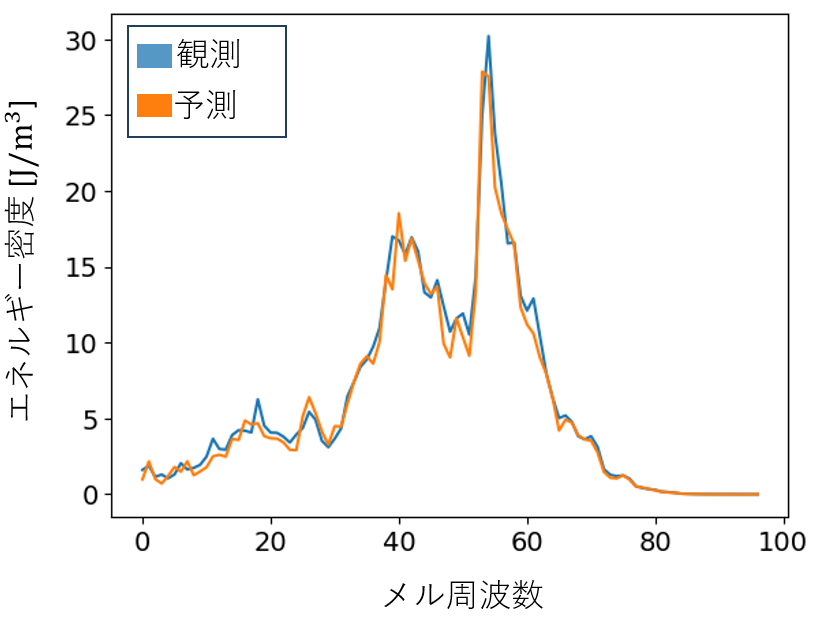
\includegraphics[keepaspectratio, width=0.7\linewidth]{chap4/comparison_pre_mel.png}
  \caption{予測されたメルスペクトログラムと観測されたメルスペクトログラムの1例}
  \label{fig:comparison_pre_mel}
\end{figure}

この図から,周波数領域におけるピークなどの正常音の特徴が正しく予測されていることが分かる.
また,これらのフレームごとの結果を横軸に結合していくことで,時間ごと特定の環境特性を示すメルスペクトログラムを得ることができる.
観測された音のメルスペクトログラムと座標に基づいて予測されたメルスペクトログラムを図\ref{fig:observed_mel}と図\ref{fig:predicted_mel}に示す.

\begin{figure}[t]
  \centering
  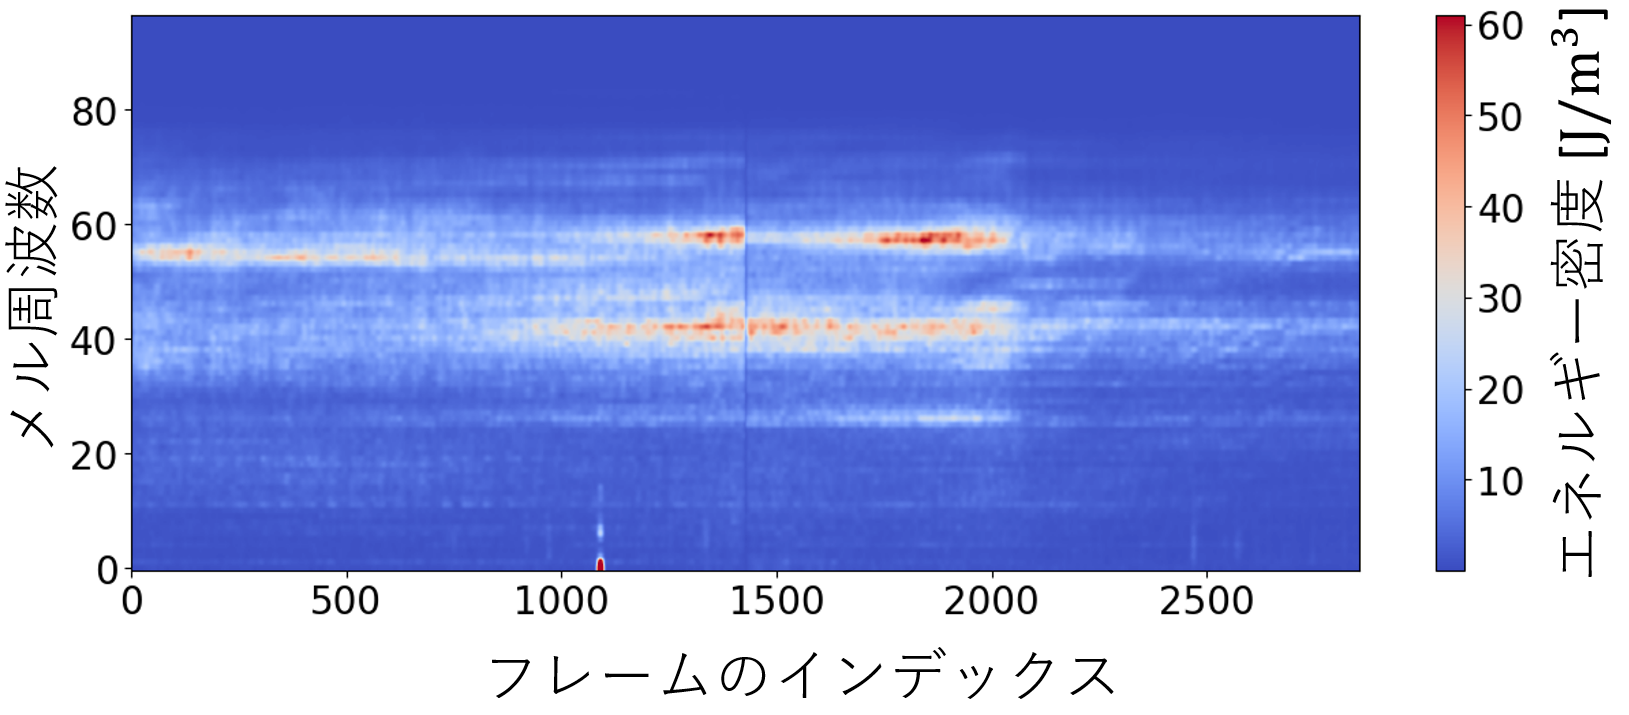
\includegraphics[keepaspectratio, width=0.7\linewidth]{chap4/observed_mel.png}
  \caption{観測されたメルスペクトログラム}
  \label{fig:observed_mel}
\end{figure}

\begin{figure}[t]
  \centering
  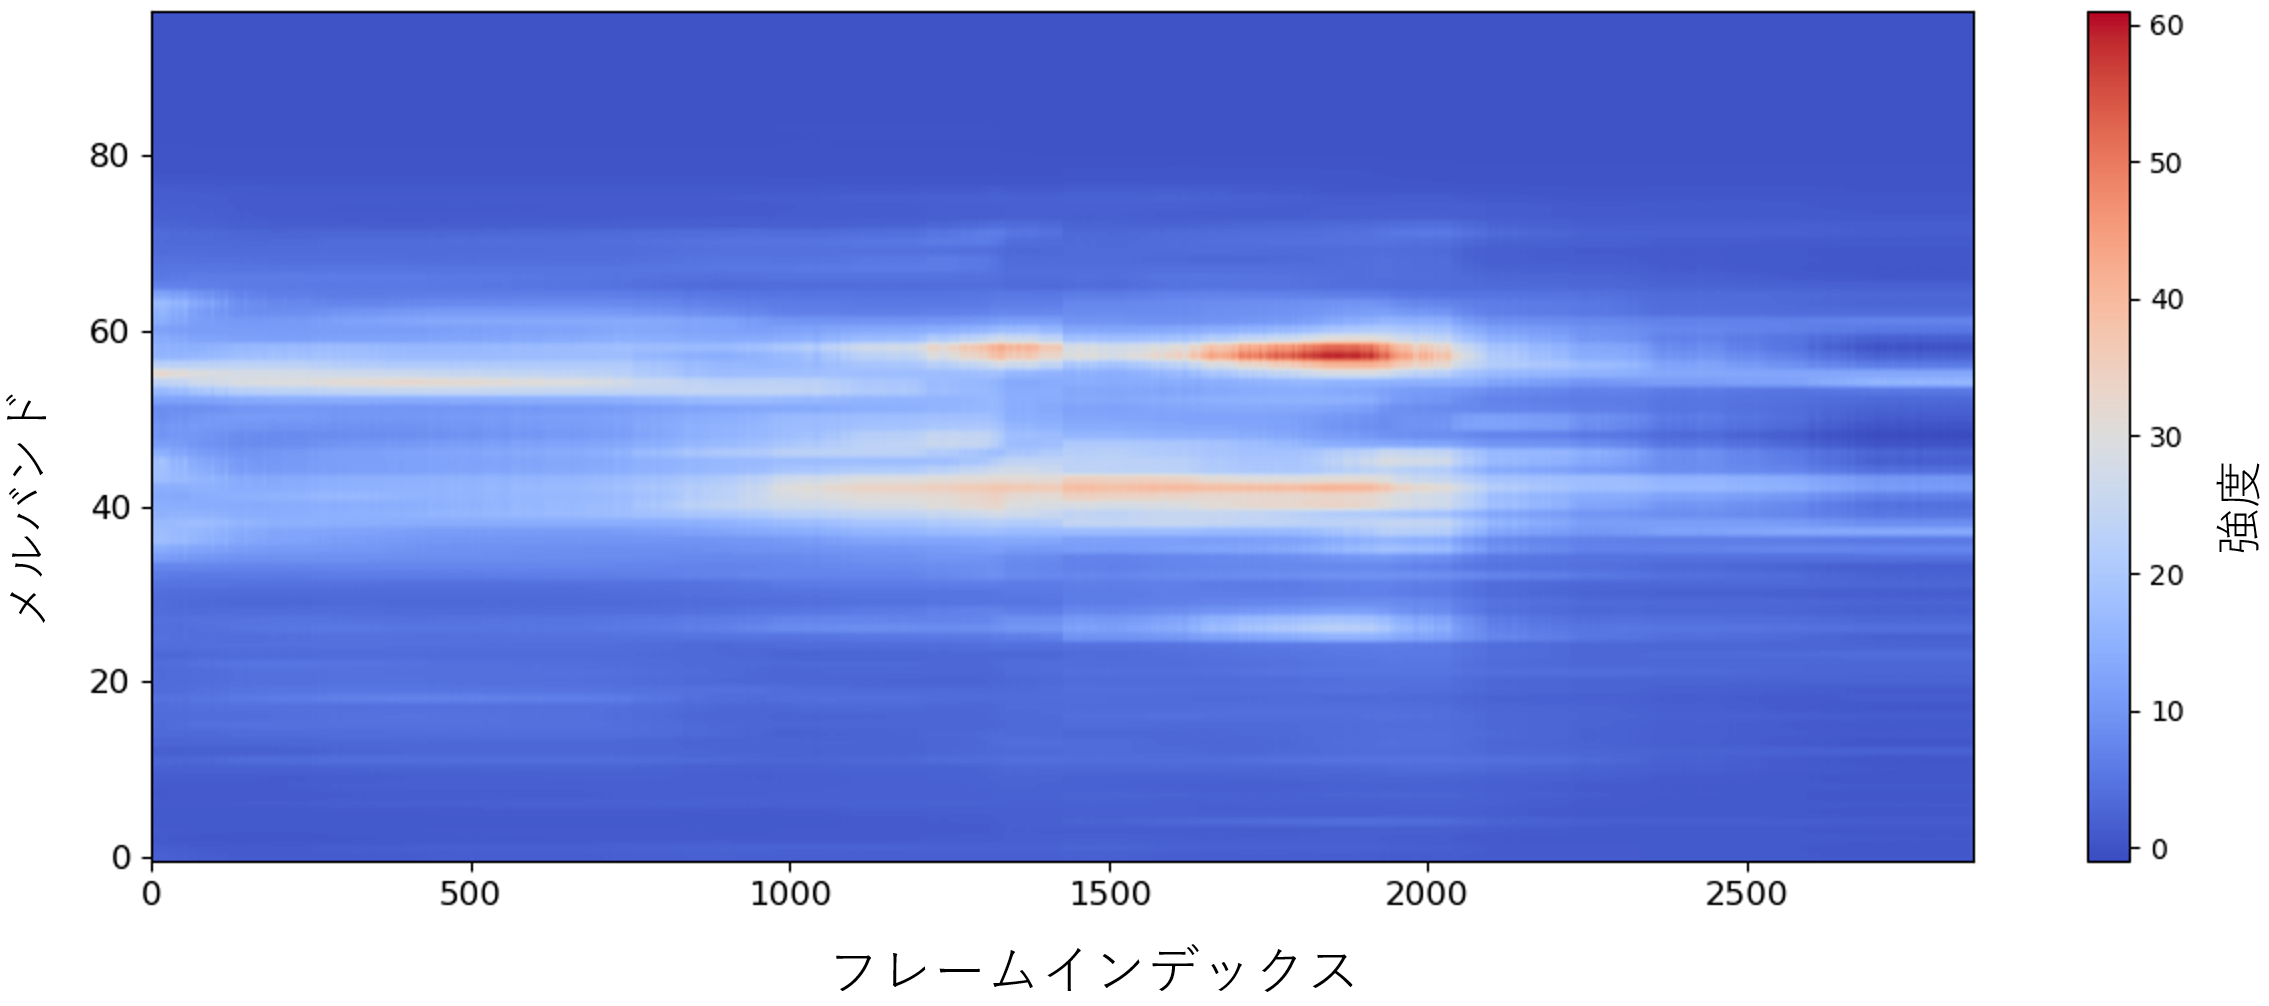
\includegraphics[keepaspectratio, width=0.7\linewidth]{chap4/predicted_mel.png}
  \caption{予測されたメルスペクトログラム}
  \label{fig:predicted_mel}
\end{figure}
図\ref{fig:observed_mel}と図\ref{fig:predicted_mel}を比較すると,殆ど全てのフレームにおいて,強度の強いメルバンドが一致しており,このことから提案手法が正常音のマッピングを適切に行っていることが分かる.

\subsubsection{異常音の検出} \label{subsubsec:anomaly_detection}
異常状態の経路は,異常のギアボックスの配置を変え,2種類の経路にて走行した.
正常状態の経路と,異常音源を設置した経路における予測音との差分エネルギー分布を図\ref{fig:lab_normal},図\ref{fig:lab_abnormal2},図\ref{fig:lab_abnormal7}に示す.
これらの図から,異常音源を設置した付近の座標ではエネルギー値が大きくなり,異常音源から離れるにつれエネルギー値が小さくなることが分かる.
これらの結果から,提案手法が異常音を検出することができることが示された.


\begin{figure}[t]
  \centering
  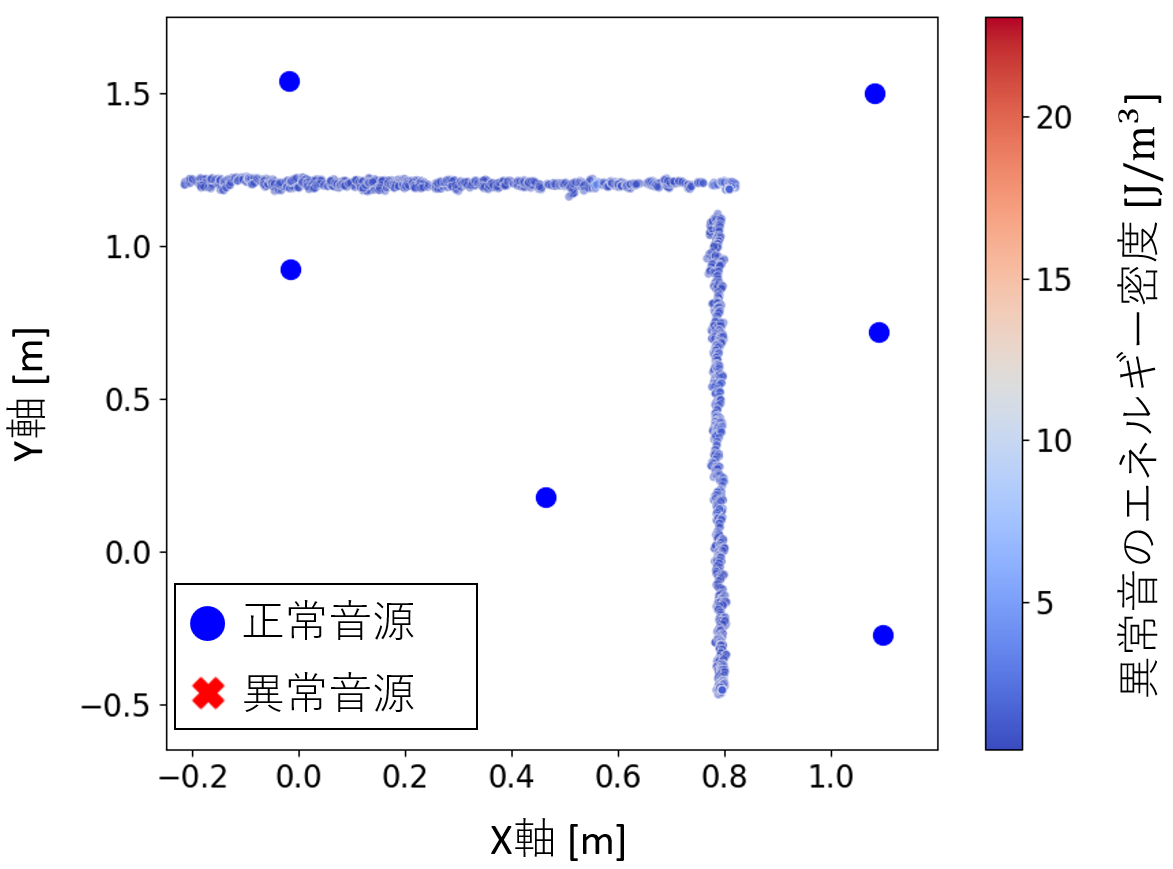
\includegraphics[keepaspectratio, width=0.7\linewidth]{chap4/lab_normal.png}
  \caption{正常状態の経路における予測音との差分エネルギーの分布}
  \label{fig:lab_normal}
\end{figure}

\begin{figure}[t]
  \centering
  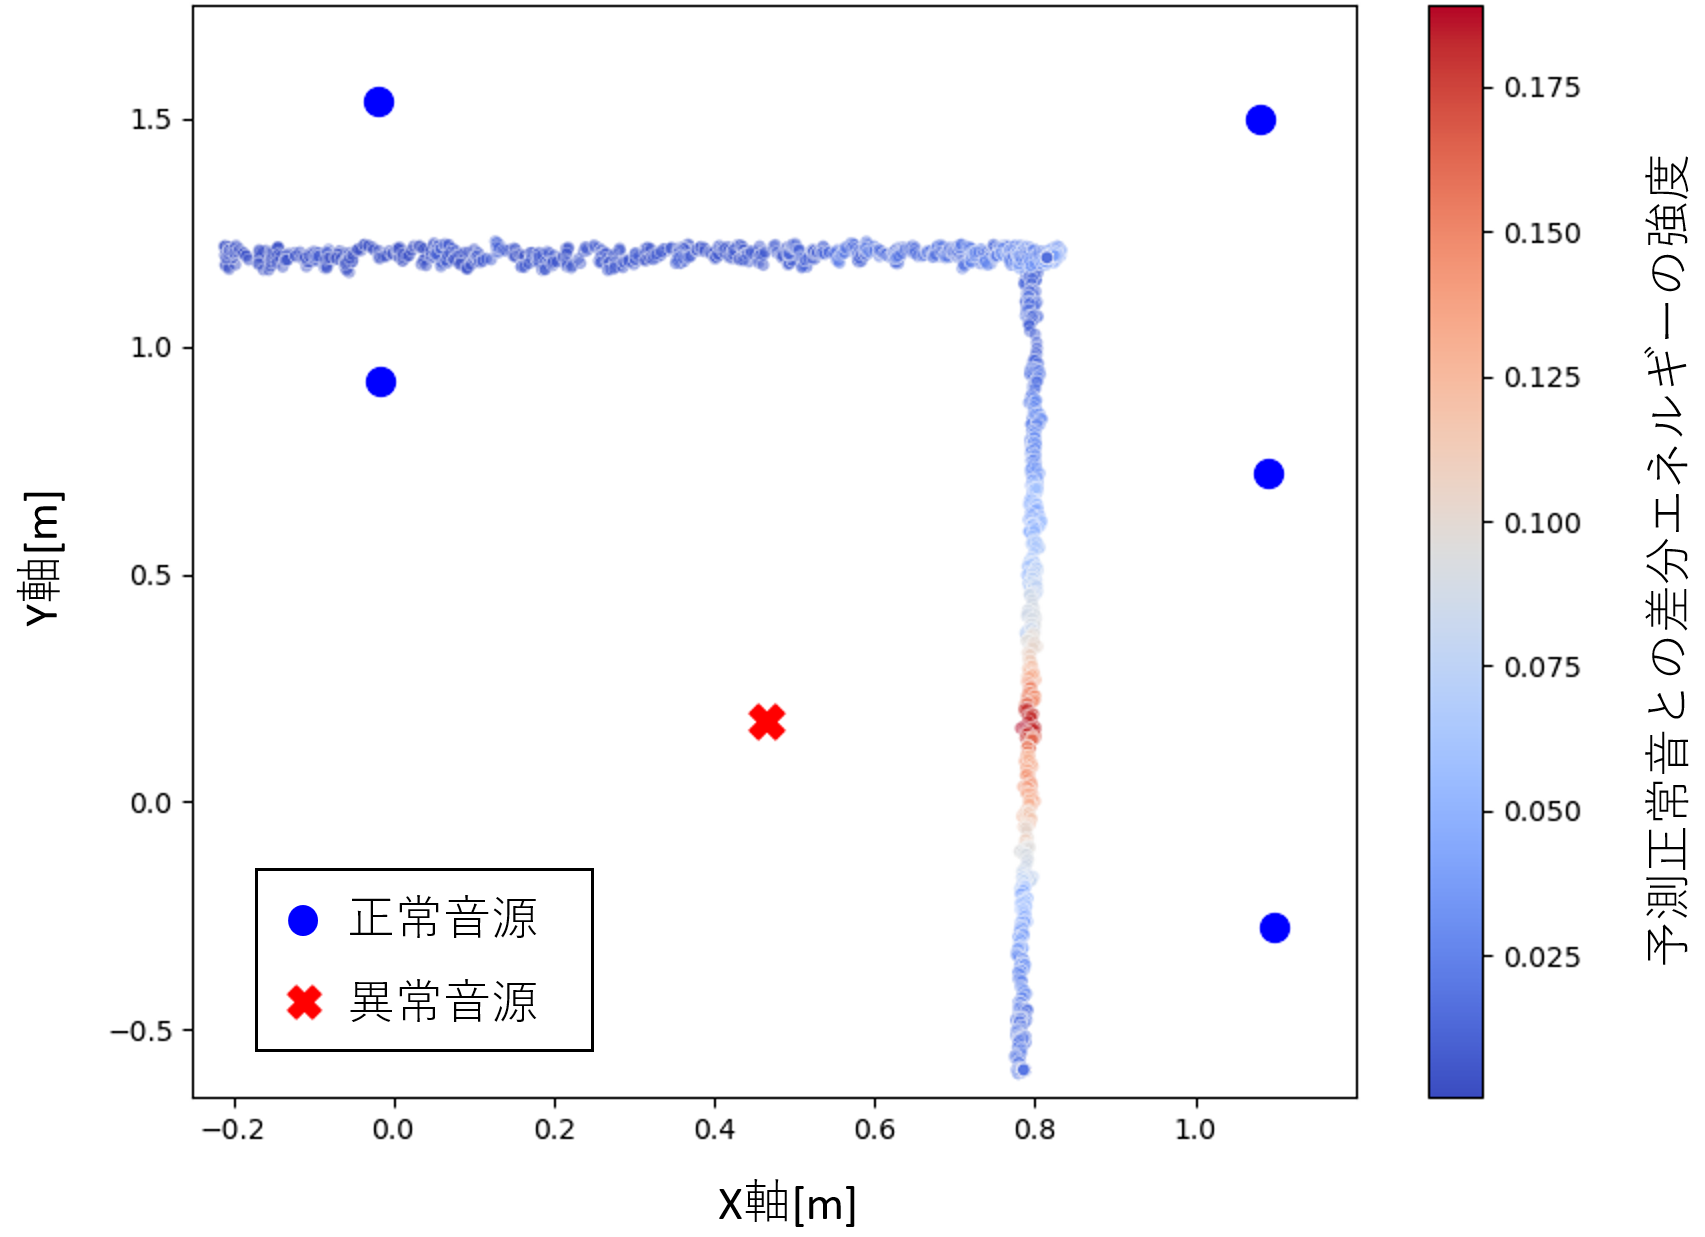
\includegraphics[keepaspectratio, width=0.7\linewidth]{chap4/lab_abnormal2.png}
  \caption{異常状態の経路における予測音との差分エネルギーの分布}
  \label{fig:lab_abnormal2}
\end{figure}

\begin{figure}[t]
  \centering
  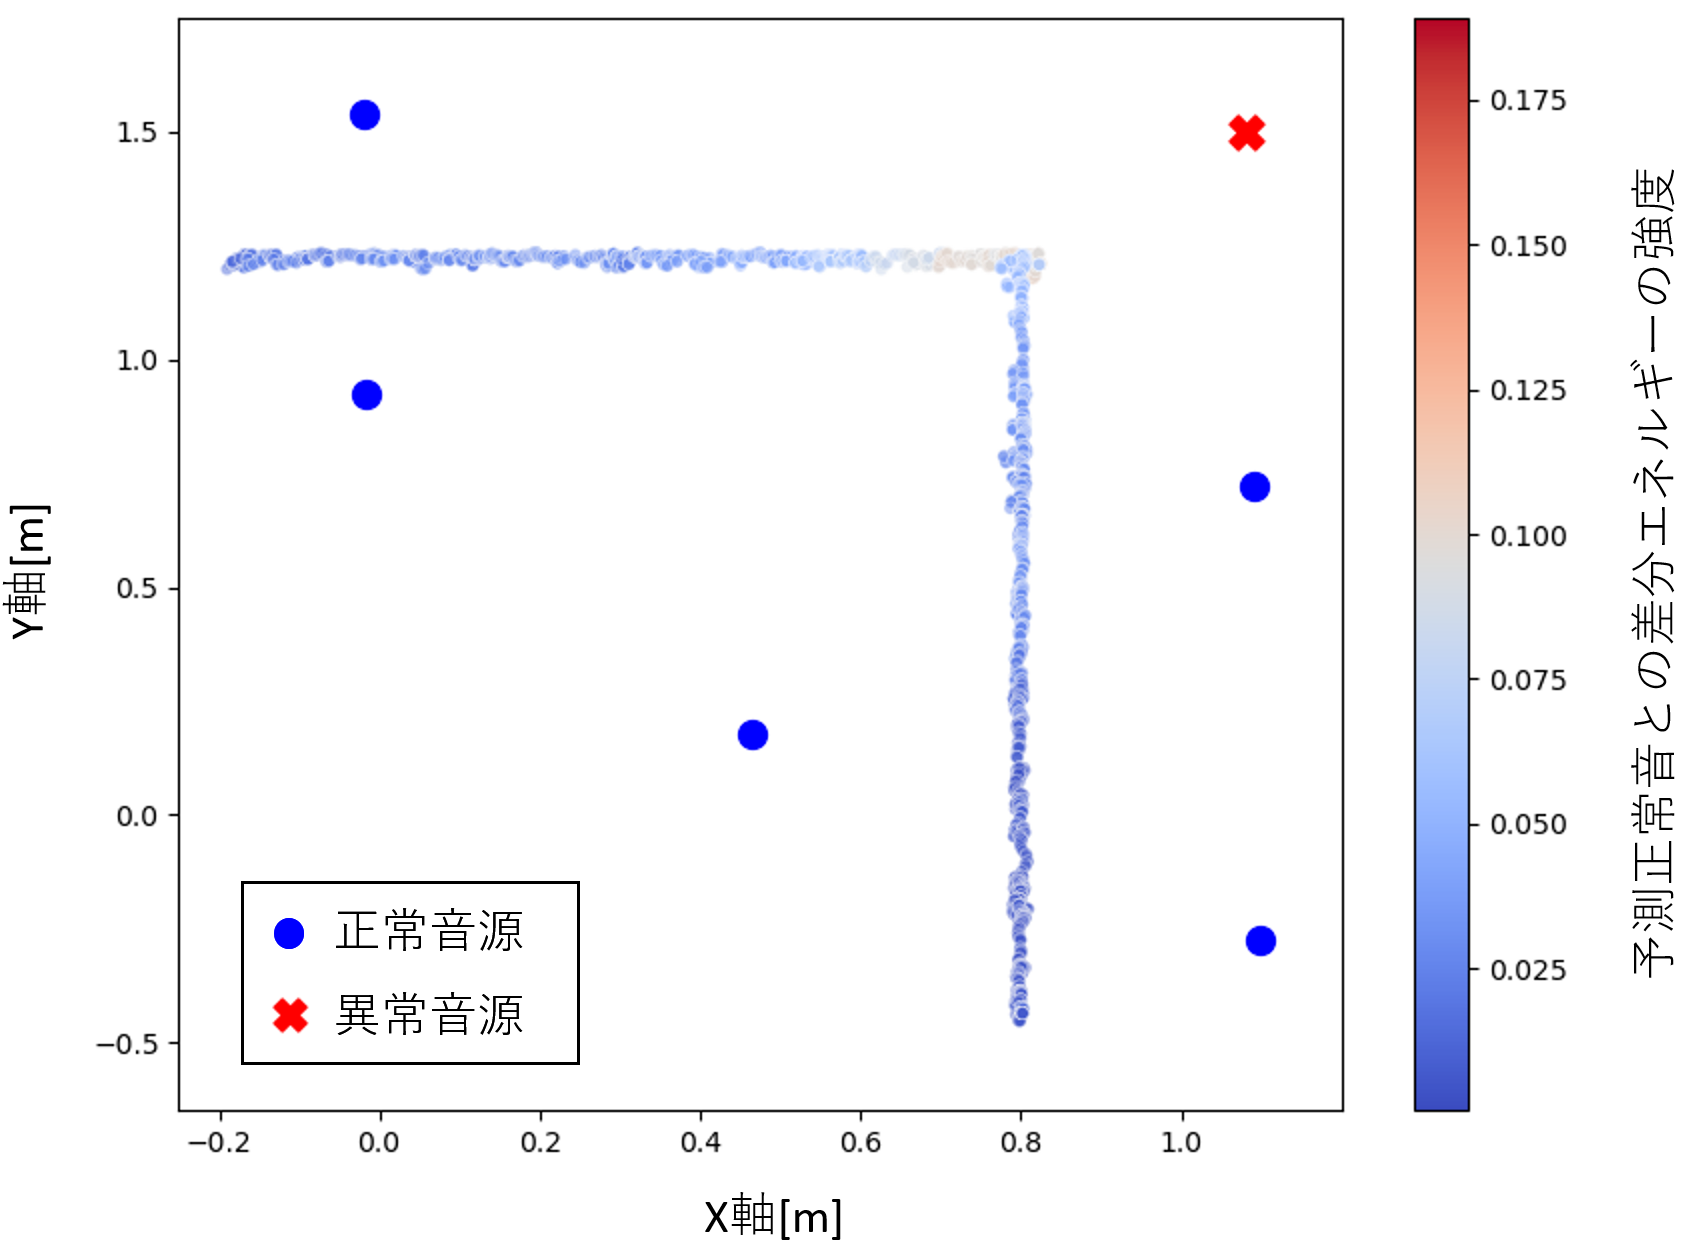
\includegraphics[keepaspectratio, width=0.7\linewidth]{chap4/lab_abnormal7.png}
  \caption{異常状態の経路における予測音との差分エネルギーの分布}
  \label{fig:lab_abnormal7}
\end{figure}

\subsubsection{異常音源の座標推定} \label{subsubsec:source_localization}

異常が検出されたエリアについて,音源の座標を推定した結果を\reftab{tab:sound_localization}に示す.
いずれのケースでも実際の異常音源の位置と推定値の誤差は小さく,高い精度で位置推定が行われていることが確認された.

\begin{table}[h]
  \centering
  \caption{提案手法による異常音源位置推定の結果}
  \label{tab:sound_localization}
  \begin{tabular}{>{\centering\arraybackslash}m{3cm} >{\centering\arraybackslash}m{4cm} >{\centering\arraybackslash}m{4cm}}
      \toprule
      & 位置1 & 位置2 \\
      \midrule
      真値 & (0.46, 0.18) & (1.08, 1.50) \\
      提案手法 & (0.55, 0.21) & (1.17, 1.45) \\
      誤差(m) & 0.09 & 0.10 \\
      \bottomrule
  \end{tabular}
\end{table}


\subsection{考察} \label{subsec:discussion}

まず,正常音のマッピングに関する考察を述べる.
\reffig{fig:comparison_pre_mel}を見ると,観測されたメルスペクトログラムは大きく分けて,3つのピークが存在していることが分かる.
それぞれ,メルバンドで20,40,55に対応しており,この順に周波数が高くなっている.
これらのピークの中で,40,55に対応する信号強度はよく予測できている.しかし,メルバンドが20付近のピークに対しては,予測されたメルスペクトログラムと観測されたメルスペクトログラムでは,ピークに対応するメルバンドが異なっている.
これは,ピークの強度の弱い部分では,ノイズの影響が大きいため,学習データもしくはテストデータにおいてノイズが含まれていることが原因と考えられる.

次に\reffig{fig:observed_mel}と\reffig{fig:predicted_mel}を比較する.
まず,\reffig{fig:observed_mel}において,ロボットの移動に応じて,信号強度の強い周波数帯が連続的に変化していることが分かる.
この連続的な変化は,\reffig{fig:predicted_mel}においても同様に観測されている.
このことから,\refsec{sec:pmethod_sequential}で述べたように音源が固定されており,それらの音源が定常的な特徴を持つ場合,観測される音はロボットの自己位置に応じて連続的に変化し,SAMアルゴリズムを用いたこの連続的な関係の学習が可能であることが示されていると考えられる.

また,\reffig{fig:observed_mel}では,フレームのインデックスが1100付近において,低周波帯にて信号強度が急激に増加していることがわかる.
このような急激な増加は,ロボットの振動によるノイズが含まれている可能性が高い.
このような急激な増加は,\reffig{fig:predicted_mel}においては観測されていないことから,このようなノイズが原因で異常音のエネルギー値が一定の箇所で急激に増加してしまう可能性がある.
本実験においては,ロボットの移動に基づくノイズの影響を受けやすい低周波帯において,特徴量をカットすることでこのようなノイズの影響を抑制したが,移動ロボットのノイズ特性に応じたノイズ低減手法の検討は今後の課題である.

次に,異常音の検出に関する結果について考察する.
\reffig{fig:lab_normal}では,全ての機器が正常に稼働しており,異常音源が存在しないためエネルギー値は経路内の全ての点において非常に小さくなっている.
一方,\reffig{fig:lab_abnormal2}と\reffig{fig:lab_abnormal7}では,異常音源が存在するエリアにおいてエネルギー値が大きくなっていることが分かる.
また,\reffig{fig:lab_abnormal2}と\reffig{fig:lab_abnormal7}を比較すると,エネルギー強度のピークの大きさと,赤くプロットされている経路内お点の数が異なることが分かる.
これは,位置1では,異常音源がL字の経路の曲がり角の内側に存在するため,比較的異常音源に近づくことができ,エネルギー値が大きくなっていることが分かる.
一方で位置2では,異常音源がL字の経路の曲がり角の外側に存在するため,異常音源に近づくことができず,エネルギー値が小さくなっていることが分かる.
この結果から,提案手法を用いて異常音の検知をする際には,異常と診断される可能性がある機器の配置に応じて正しく経路を設定することが重要であることが考えられる.


最後に,異常音源の位置推定に関する結果について考察を述べる.
\reftab{tab:sound_localization}に示すように,提案手法による異常音源の位置推定は,真値との誤差が小さく,高い精度で位置推定が行われていることが示された.
また,\reffig{fig:lab_abnormal2}と\reffig{fig:lab_abnormal7}では,検出されたピークの異常音エネルギーのにおいて差が見られたが,位置1と位置2において,異常音源の位置推定精度に大きな差は見られなかった.
このことから,提案手法を用いた異常音源の位置推定は,異常音源の位置に対して頑健であることが分かった.これは最適化において異常音のエネルギーの大きさをもとに重み付けをしているため,経路を通じた異常音のエネルギーが小さい場合にも,その経路の中で相対的に大きなエネルギーを持つ点の情報を正しく利用することができているためだと考えられる.

\end{document}
